\begin{center}
    {\LARGE\bfseries Решения заключительного отбора Сириус 8 класс 2026 год.}\\[2mm]
\end{center}

\problem{1}
Найти цифры $a,b$ и натуральное $m$, если $5(2m+1)(2m+3)(2m+5)=ababab$,
где $ababab$ -- шестизначное число с чередующимися цифрами $a$ и $b$.

\textit{Решение.}
Запишем число $ababab$ в удобном виде: $ababab=10101(10a+b).$
Положим $x=2m+3.$ Тогда $5(x-2)x(x+2)=10101(10a+b).$ Так как $10101=3\cdot 7\cdot 13\cdot 37$. и $\text{НОД}(5,10101)=1$, число $10a+b$ делится на $5$, а произведение $(x-2)x(x+2)$ делится на $10101$. Числа $x-2$, $x$, $x+2$ нечётные и попарно взаимно простые. Кроме того, из неравенства $5(x-2)x(x+2)\le 999999$  получаем $x\le 57$, потому что при $x\ge 59$ уже $5\cdot 57\cdot 59\cdot 61>999999.$ Значит, среди чисел $x-2$, $x$, $x+2$ кратным $37$ может быть только само число $37$. Поэтому возможны только три случая: $x-2=37,x=37, x+2=37.$ То есть $x=39, x=37, x=35.$ Проверим их. Если $x=35$, то $(x-2)x(x+2)=33\cdot 35\cdot 37,$ и множителя $13$ нет. Если $x=39$, то $(x-2)x(x+2)=37\cdot 39\cdot 41,$ и множителя $7$ нет. Остаётся $x=37.$ Тогда $2m+3=37,$ откуда $m=17.$ Подставляем: $5\cdot 35\cdot 37\cdot 39=252525.$ Значит, $a=2, b=5.$

\textit{Ответ: $a = 2, b = 5$}

\problem{2}
За круглым столом сидит $n$ человек: рыцари и лжецы. Каждый говорит, что через два человека левее него сидит рыцарь. Известно, что есть и рыцари, и лжецы. Может ли $n=2026$?

\textit{Решение.}
Пронумеруем людей от 1 до 2026. Пусть 1-й человек рыцарь. Тогда \\ $4, 7, \ldots, 2026$ тоже рыцари. Но если 2026-й рыцарь, то и 3-й тоже рыцарь. Тогда и $6, 9, \ldots, 2025$ тоже рыцари. Но если 2025-й рыцарь, то и 2-й тоже рыцарь. Наконец тогда $5, 8, \ldots 2024$ тоже рыцари, а значит все люди рыцари. Но по условию есть и те и другие. Значит 2026 людей сидеть не могло.

\problem{3}
Змей ходит на соседние клетки как король и ещё на $2$ клетки по диагонали. Сколько максимум можно разместить змеев, чтобы они не били друг друга?

\newpage

\hspace{3mm}

\textit{Решение.} Сначала покажем как расположить 14 змей.

\begin{figure}[h]
    \centering
    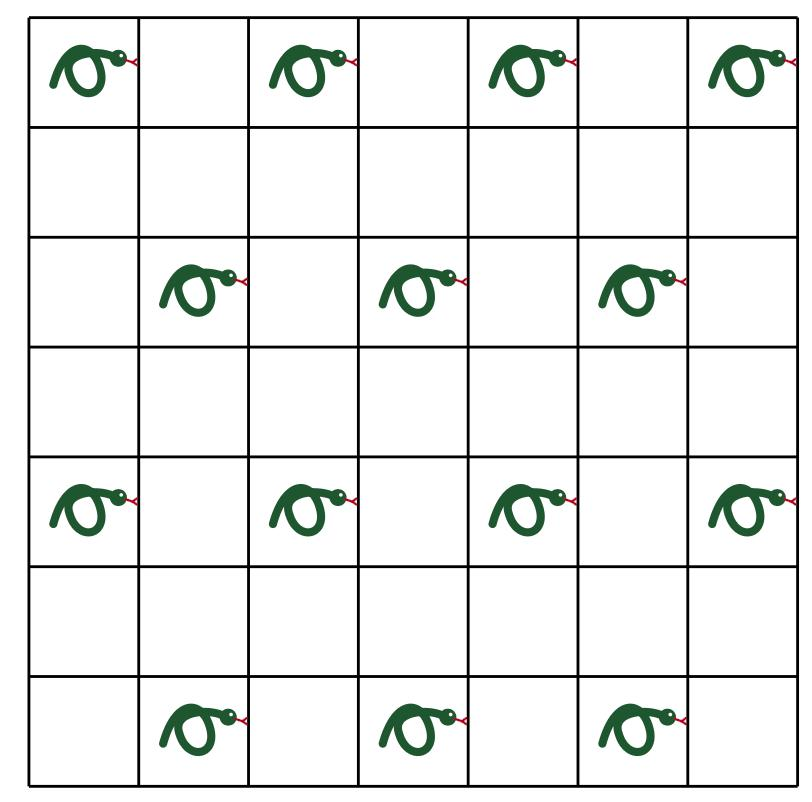
\includegraphics[width=0.3\linewidth]{ЭлМШ 2025-2026/разбор Сириуса/8/snakes_example.jpg}
    \caption{Пример на 14 змей}
    \label{fig:placeholder}
\end{figure}

А эта картинка доказывает, что больше 14 змей расставить не получится. Действительно, в каждую группу клеток можно поставить не более одной змеи, а групп всего 14. 

\begin{figure}[h]
    \centering
    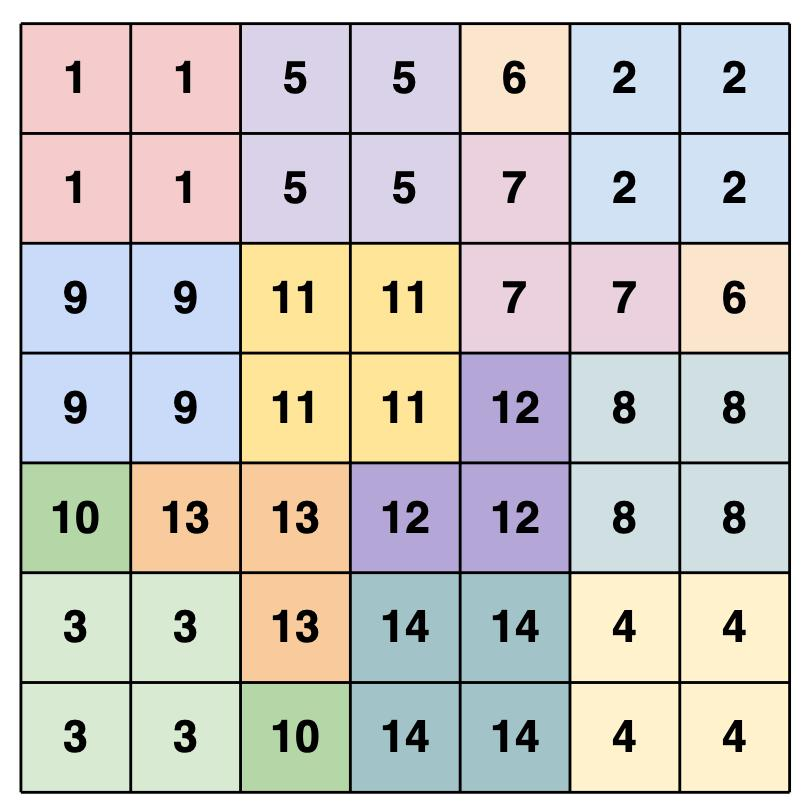
\includegraphics[width=0.3\linewidth]{ЭлМШ 2025-2026/разбор Сириуса/8/snakes_groups.jpg}
    \caption{Разбиение на группы}
    \label{fig:placeholder}
\end{figure}

\problem{4}
Пусть $k>1013$ и
\[
a_1<a_2<a_3<\dots<a_k\le 2026.
\]
Докажите, что найдутся $a_m,a_n$, для которых
\[
a_1+a_m=a_n.
\]

\textit{Решение.}
Обозначим $d=a_1$. Предположим противное: для любых $m,n$ не выполнено $a_1+a_m=a_n$, то есть среди чисел $a_1,\ldots,a_k$ нет двух, отличающихся на $d$. Так как все $a_i$ лежат на отрезке $[d,2026]$, причём $k>1013$, имеем $2027-d\ge k>1013$, откуда $d\le 1013$. Разобьём все числа от $d$ до $2026$ на $d$ арифметических прогрессий с разностью $d$:
\[
d,2d,3d,\ldots;\qquad d+1,2d+1,3d+1,\ldots;\qquad \ldots;\qquad 2d-1,3d-1,4d-1,\ldots,
\]
обрывая каждую прогрессию на числе, не превосходящем $2026$. Пусть их длины равны $\ell_1,\ldots,\ell_d$. Внутри каждой такой прогрессии нельзя выбрать два соседних числа, поскольку они отличаются ровно на $d$. Поэтому из прогрессии длины $\ell_i$ можно выбрать не более $\left\lceil \frac{\ell_i}{2}\right\rceil$ чисел. Значит,
\[
k\le \sum_{i=1}^d \left\lceil \frac{\ell_i}{2}\right\rceil
=\frac{\ell_1+\cdots+\ell_d+s}{2},
\]
где $s$ --- количество нечётных среди чисел $\ell_1,\ldots,\ell_d$. Но
\[
\ell_1+\cdots+\ell_d=2027-d.
\]
Кроме того, $s\le d-1$: действительно, все $d$ длин не могут быть нечётными, потому что тогда их сумма имела бы ту же чётность, что и $d$, тогда как число $2027-d$ имеет противоположную чётность. Следовательно,
\[
k\le \frac{2027-d+d-1}{2}=1013,
\]
что противоречит условию $k>1013$. Значит, предположение неверно, и найдутся $a_m,a_n$, для которых
\[
a_1+a_m=a_n.
\]

\problem{5}
Дан выпуклый пятиугольник $АВСDE$. Известно, что $AB = AE, BC = CD, \angle E = \angle D = 90^{\circ},$ биссектрисы углов $A$ и $C$ пересекаются в точке $I$, точка $M$ середина отрезка $AC$. Доказать, что угол $\angle MIC = \angle AIB$.

\textit{Решение 1(Дорджиев Арлтан).}
Пусть \(F\) и \(S\) --- середины \(ED\) и \(EB\) соответственно. Из \(AB=AE\) следует, что в равнобедренном \(\triangle ABE\) биссектриса \(AI\) является серединным перпендикуляром к \(BE\), то есть \(A,I,S\) лежат на одной прямой и \(IS\perp BE\). Аналогично, из \(CB=CD\) получаем \(CI\perp BD\). Поэтому \(I\) равноудалена от \(B,E,D\), а значит, является центром описанной окружности \(\triangle EBD\). Следовательно, \(IF\perp ED\).

Так как \(\angle AED=\angle CDE=90^\circ\), то \(AE\parallel CD\). В трапеции \(AECD\) точки \(F\) и \(M\) --- середины боковых сторон \(ED\) и \(AC\), значит, \(FM\parallel AE\). Но \(IF\perp ED\) и \(AE\perp ED\), откуда \(IF\parallel AE\). Следовательно, \(I,F,M\) лежат на одной прямой.

В \(\triangle EBD\) отрезок \(SF\) --- средняя линия, поэтому \(SF\parallel BD\). Кроме того, \(IS\perp EB\) и \(IF\perp ED\), значит, \(\angle ISE=\angle IFE=90^\circ\), то есть \(ISFE\) --- вписанный четырёхугольник. Так как \(IE=IB\), а \(S\) --- середина \(EB\), то \(IS\) --- биссектриса \(\angle EIB\), поэтому
\[
\angle AIB=\angle EIS=\angle EFS=\angle EDB.
\]
С другой стороны, \(MI\parallel IF\perp ED\) и \(IC\perp BD\), значит,
\[
\angle MIC=\angle EDB.
\]
Следовательно, \(\angle MIC=\angle AIB\).

\begin{figure}[h]
    \centering
    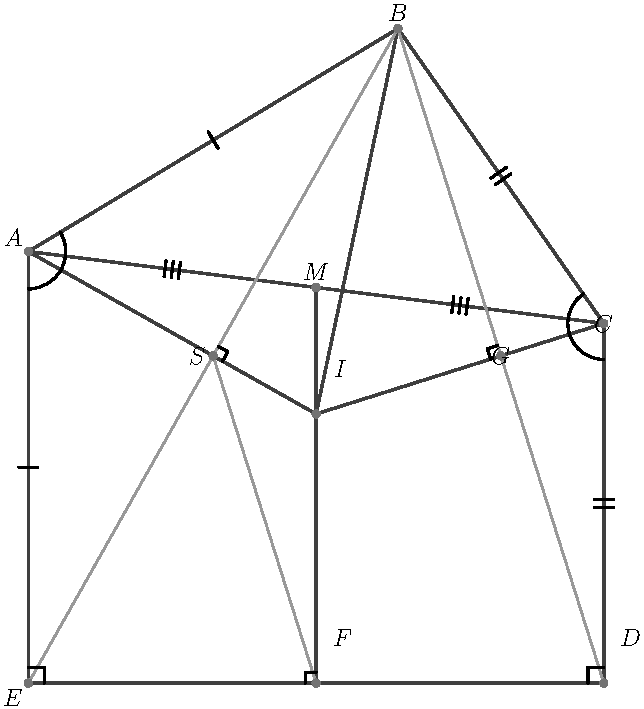
\includegraphics[width=0.5\linewidth]{ЭлМШ 2025-2026/разбор Сириуса/8/pentagon_bisectors.pdf}
    \caption{Enter Caption}
    \label{fig:placeholder}
\end{figure}

\textit{Решение 2 (изогональное сопряжение).}
Из \(AB=AE\) и \(CB=CD\) получаем, что \(AI\) и \(CI\) --- серединные перпендикуляры к хордам \(BE\) и \(BD\) одной окружности с центром \(I\). Кроме того, из \(AE\parallel CD\) и того, что \(M\) --- середина \(AC\), следует, что \(IM\) --- серединный перпендикуляр к \(DE\). Пусть направления \(IB,ID,IE\) равны \(b,d,e\). Тогда направления серединных перпендикуляров к хордам \(XY\) равны полусуммам направлений \(IX\) и \(IY\), поэтому
\[
AI=\frac{b+e}{2},\qquad CI=\frac{b+d}{2},\qquad IM=\frac{d+e}{2}.
\]
Следовательно,
\[
AI+CI=IB+IM,
\]
то есть \(IB\) и \(IM\) изогональны в угле \(\angle AIC\). Значит, \(\angle AIB=\angle MIC\).

\textit{Решение 3 (декартовы координаты).}
Снова имеем: \(AI\) --- серединный перпендикуляр к \(BE\), \(CI\) --- серединный перпендикуляр к \(BD\), поэтому \(I\) --- центр окружности \((BDE)\). Также, если \(F\) --- середина \(ED\), то из \(AE\parallel CD\) получаем, что \(MF\) --- средняя линия трапеции \(AECD\), значит, \(MF\parallel AE\perp ED\). Следовательно, \(I,F,M\) лежат на серединном перпендикуляре к \(ED\).

Возьмём декартову систему координат с началом в \(I\), а окружность \((BDE)\) сделаем единичной. Пусть
\[
B=(\cos\beta,\sin\beta),\qquad D=(\cos\delta,\sin\delta),\qquad E=(\cos\varepsilon,\sin\varepsilon).
\]
Для хорды с концами
\[
X=(\cos x,\sin x),\qquad Y=(\cos y,\sin y)
\]
её середина имеет координаты
\[
\left(\frac{\cos x+\cos y}{2},\frac{\sin x+\sin y}{2}\right)
=\cos\frac{x-y}{2}\left(\cos\frac{x+y}{2},\sin\frac{x+y}{2}\right),
\]
поэтому серединный перпендикуляр к хорде \(XY\) имеет направление \(\frac{x+y}{2}\) по модулю \(\pi\). Значит,
\[
\dir IA=\frac{\beta+\varepsilon}{2},\qquad
\dir IC=\frac{\beta+\delta}{2},\qquad
\dir IM=\frac{\delta+\varepsilon}{2},\qquad
\dir IB=\beta.
\]
Тогда для ориентированных углов получаем
\[
\angle AIB=\beta-\frac{\beta+\varepsilon}{2}=\frac{\beta-\varepsilon}{2},
\]
а также
\[
\angle MIC=\frac{\beta+\delta}{2}-\frac{\delta+\varepsilon}{2}=\frac{\beta-\varepsilon}{2}.
\]
Следовательно,
\[
\angle MIC=\angle AIB.
\]

\textit{Решение 4 (комплексные координаты).}
Пусть \(F\) --- середина \(ED\). Как и раньше, из \(AB=AE\) и \(CB=CD\) следует, что \(AI\) и \(CI\) являются серединными перпендикулярами к \(BE\) и \(BD\) соответственно. Поэтому \(IB=IE=ID\), то есть \(I\) --- центр окружности, проходящей через \(B,D,E\). Кроме того, \(AE\parallel CD\), значит, в трапеции \(AECD\) отрезок \(MF\) является средней линией, откуда \(MF\parallel AE\). Так как \(AE\perp ED\), то \(MF\perp ED\), а значит, \(IM\) является серединным перпендикуляром к \(ED\).

Поместим теперь точку \(I\) в начало комплексной плоскости, а окружность \((BDE)\) сделаем единичной. Пусть точкам \(B,D,E\) соответствуют комплексные числа \(b,d,e\), где \(|b|=|d|=|e|=1\). Для хорды с концами \(x,y\) серединный перпендикуляр имеет направление
\[
\arg(x+y)=\frac{\arg x+\arg y}{2}\pmod\pi.
\]
Следовательно,
\[
\arg IA=\frac{\arg b+\arg e}{2},\qquad 
\arg IC=\frac{\arg b+\arg d}{2},\qquad
\arg IM=\frac{\arg d+\arg e}{2},\qquad
\arg IB=\arg b .
\]
Тогда
\[
\arg IA+\arg IC
=\frac{\arg b+\arg e}{2}+\frac{\arg b+\arg d}{2}
=\arg b+\frac{\arg d+\arg e}{2}
=\arg IB+\arg IM \pmod\pi.
\]
Значит, прямые \(IB\) и \(IM\) изогональны относительно угла \(\angle AIC\), то есть
\[
\angle MIC=\angle AIB.
\]


\problem{6}
В связном графе без циклов есть $2026$ вершин степени хотя бы $5$. Найдите минимальное количество вершин в этом графе.

\textit{Решение.}
Связный граф без циклов -- это дерево.

Пусть в дереве $L$ листьев, то есть вершин степени $1$. Для любого дерева верна формула
\[
L=2+\sum_{\deg v\ge 2}(\deg v-2). \tag{1}
\]
Докажем её коротко. Пусть всего в дереве $V$ вершин. Тогда сумма степеней равна
\[
2(V-1).
\]
Если отделить листья, то
\[
L+\sum_{\deg v\ge 2}\deg v=2(V-1).
\]
Поскольку
\[
V=L+\#\{v:\deg v\ge 2\},
\]
после переноса слагаемых получаем ровно формулу (1).

Теперь в нашем дереве есть $2026$ вершин степени хотя бы $5$. Каждая такая вершина даёт в сумму (1) вклад не меньше
\[
5-2=3.
\]
Поэтому
\[
L\ge 2+2026\cdot 3=6080.
\]
Кроме этих листьев, в дереве есть ещё как минимум $2026$ вершин степени хотя бы $5$. Значит, общее число вершин не меньше
\[
6080+2026=8106. \tag{2}
\]

Осталось показать, что эта оценка достижима. Возьмём путь на $2026$ вершинах. У двух концов степень $1$, у остальных $2024$ вершин степень $2$. Довесим к каждой вершине пути столько новых листьев, чтобы её степень стала ровно $5$.

К двум концам нужно добавить по $4$ листа, а к каждой из $2024$ внутренних вершин -- по $3$ листа. Всего добавлено
\[
2\cdot 4+2024\cdot 3=8+6072=6080
\]
листьев. В получившемся дереве ровно $2026$ вершин степени $5$, а всего вершин
\[
2026+6080=8106.
\]
Значит, меньше быть не может, и $8106$ действительно достигается.

\textit{Ответ: 8106}